git\documentclass[12pt, a4paper]{article}
\usepackage{lmodern}
%\usepackage[margin=1cm]{geometry}
\usepackage{pdflscape}
\usepackage{color}
\usepackage{footnote}
\usepackage{graphicx}
%\pagestyle{empty}

\definecolor{darkgreen}{rgb}{0.01, 0.75, 0.24}

\newcommand{\cell}[2][c]{%
  \begin{tabular}[#1]{@{}c@{}}#2\end{tabular}}
\newcommand{\rowhead}[2]{\cell{\color{red}#1\\ \color{darkgreen}#2}}
\newcommand{\cont}[5]{\cell{\color{red}#1\\ \color{blue}#2\\ #3\\ #4\\ \color{darkgreen}#5}}
\newcommand{\deprecont}[5]{\cell{\color{red}#1\\ \color{blue}#2\\ #3\\ #4\\ \color{darkgreen}#5\\ \color{red}Deprecated warning}}
\newcommand{\noacc}{No accumulation}
\newcommand{\acc}{Accumulation}
\newcommand{\noconv}{No conversion}
\newcommand{\sca}{Scaling possible}
\newcommand{\nosca}{Scaling not possible}
\newcommand{\conv}{Conversion}
\newcommand{\serfal}{Service=false}
\newcommand{\sertru}{Service=true}
\newcommand{\err}{\color{red}Error}
\newcommand{\depre}{\color{red}Deprecated}
\newcommand{\follsup}{Following supports $S_{R+1}\dots S_i\dots S_N$}
\newcommand{\allsup}{All supports $S_1\dots S_i\dots S_N$}
\newcommand{\modlen}{moduleLength}
\newcommand{\modsur}{moduleSurface}
\newcommand{\nummod}{numModules}
\newcommand{\suplen}{supportLength}
\newcommand{\supsur}{supportSurface}
\newcommand{\tkl}{tkLayout}

\newcommand{\pat}[1]{\texttt{#1}}
\newcommand{\prop}[1]{\texttt{#1}}


\begin{document}
\section{Introduction to material model}
The material inside \tkl is present inside the modules (i.e. silicon
and cooling blocks),
and outside the modules (i.e. cables or cooling pipes). Is possible to
specify, in the configuration files, the material inside:
\begin{itemize}
\item modules;
\item rods (the ladders);
\item barrel's layers;
\item endcap's disks;
\item custom cylinders and disks (i.e. for the supports).
\end{itemize}
Is also possible to set material from every element:
\begin{itemize}
\item locally,
\item exiting.
\end{itemize}

\begin{figure}[hbtp]
  \centering
  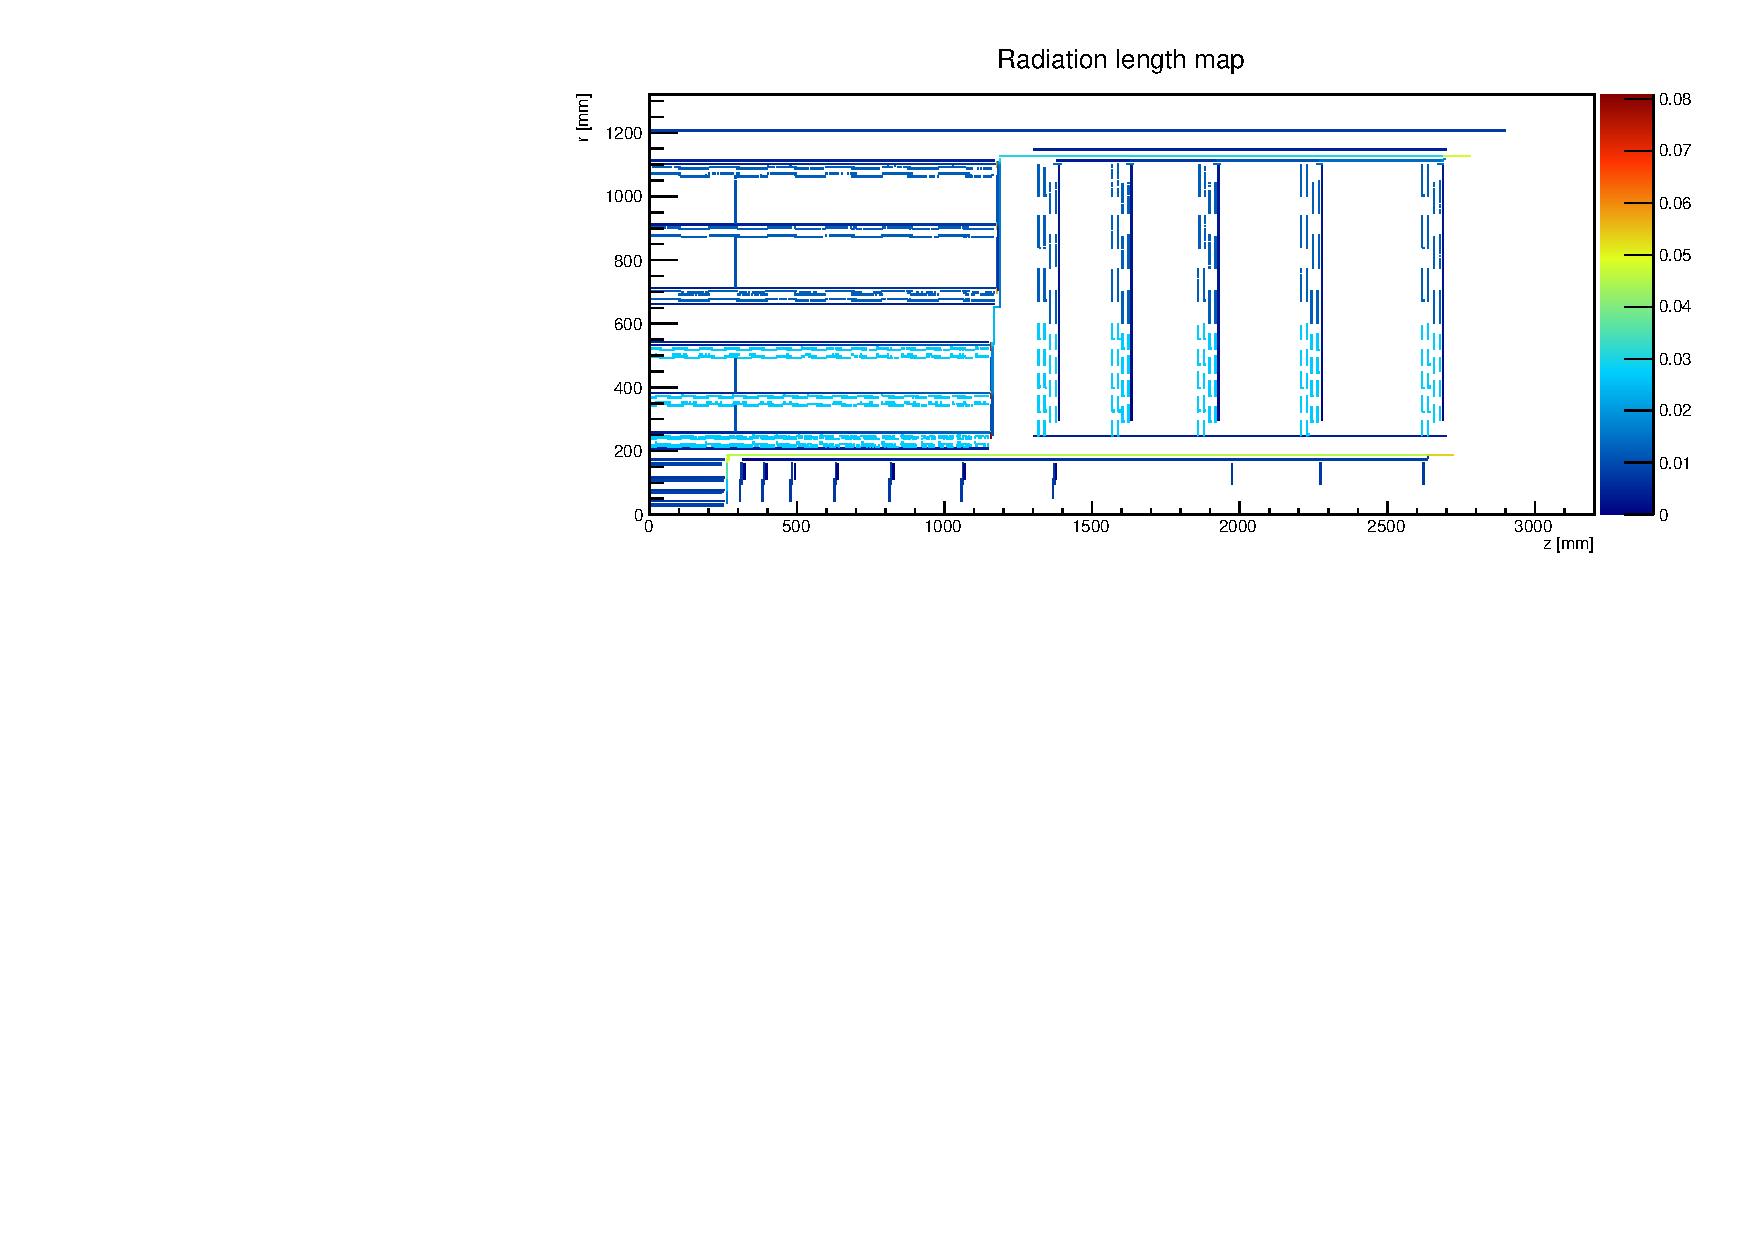
\includegraphics[width=\textwidth]{img/materialMap.pdf}  
  \caption{Material routing}
  \label{fig:materialMap}
\end{figure}

Apart from the material is possible also to define \emph{conversions}
in special points: at the end of the layers, at the end of the disks,
and in custom positon along the way.

In figure~\ref{fig:materialMap}
is visible the material for the modules and the \emph{sections} for
the routing of the material, section~\ref{sec:userManual} deal with
the description in detail of how to build the configuration files and
how the material is distributed, from an user point of view.

The material \emph{routing algorithm} builds automatically all the necessary structures for
keeping all the materials that not belongs to the modules. It builds
\emph{sections} on top of the layers, and on the right of the disks,
then connect those sections for each barrel and endcap, then connect
barrels and endcaps with the cable exit point (upper right point of
tracker). Section~\ref{sec:developerManual} deal with the description
in detail of the routing algorithm from a developer point of view.




\section{User manual}\label{sec:userManual}
\subsection{Configuration files}
The configuration files regarding the material are located in the main
configuration directory, inside:
\begin{itemize}
\item \pat{config/stdinclude/Materials/} for the definition of the
  materials;
\item \pat{config/stdinclude/Conversion/} for the definition of the
  \emph{conversions}.
\end{itemize}

In the \emph{geometry} files, the \emph{materials} should be included
at \emph{layer/disk} level, at \emph{rod} level or at \emph{module}
level, depending of the type of materials. The \emph{conversions}
instead should be included at \emph{layer} or \emph{disk} level. Like
all the properties, also for the materials is possible to define them before
the correct level and them are propagated downward.

\begin{figure}[hbtp]
\begin{verbatim}
...
Barrel TB2S {
  @includestd ModuleTypes/pt2S
  @includestd Materials/pt2S_320_18
  @includestd Materials/rodPt2S
  @includestd Conversions/flangeTB2S

  dsDistance 1.8
  Layer 1 { triggerWindow 9 }
...
\end{verbatim}
\caption{\pat{geometries/.../Baseline2015.cfg}}
\label{fig:geofile}
\end{figure}
In figure~\ref{fig:geofile} is possible to see a fragment of a
geometry configuration file with the inclusion of \emph{material} and
\emph{conversion} files.
\begin{figure}[hbtp]
\begin{verbatim}
...
Materials module-pt2S_320_40 {
  type module

  // Default sensor:
  ReferenceSensor 1 {
    numStripsAcross 1016
    numSegments 2
  }
  ReferenceSensor 2 {
    numStripsAcross 1016
    numSegments 2
  } 

  // Sensor and hybrid stuff
  // Sensor
  Component {
    componentName "2S Sensors"
    service false
    scaleOnSensor 0
    Element {
      elementName SenSi
      quantity 0.2
      unit mm
      targetVolume 1
    }
  }
...
\end{verbatim}
\caption{\pat{config/.../Materials/pt2S\_320\_40}}
\label{fig:matPt2sFile}
\end{figure}
Figure~\ref{fig:matPt2sFile} is the definition of a \emph{module}
material, with \emph{reference sensors} for the scaling.
\begin{figure}[hbtp]
\begin{verbatim}
...
Materials rodPt2S {
  type rod

  // Cooling for the module
  Component {
    componentName Cooling
    service true
    scaleOnSensor 0
    Element {
      elementName Steel
      quantity 10.29
      unit g/m
    }
    Element {
      elementName CO2
      quantity 6.28
      unit g/m
    }
  }
...
\end{verbatim}
\caption{\pat{config/.../Materials/rodPt2S}}
\label{fig:matRodPt2sFile}
\end{figure}
Figure~\ref{fig:matRodPt2sFile} is the definition of material inside
the barrel rods.
\begin{figure}[hbtp]
\begin{verbatim}
...
Station {
  stationName flangeTB2S
  type flange
...
  Conversion {
    Input {
      Element {
        elementName Cu_MV
        quantity 10
        unit g/m
      }
    }
    Output {
      Element {
        elementName Cu
        quantity 10
        unit g/m
        service true
      }
      Element {
        elementName Cu
        quantity 0.423
        unit g
        service false
      }
      Element {
        elementName PE
        quantity 0.371
        unit g
        service false
      }
    }
  }
...
\end{verbatim}
\caption{\pat{config/.../Conversions/flangeTB2S}}
\label{fig:convFlangeFile}
\end{figure}
Figure~\ref{fig:convFlangeFile} is a definition of a flange
conversion.

Let's analyze more in detail the structure of the configuration files.

\paragraph{Material configuration file}
The material configuration files have a structure made of
\emph{components} blocks with inside \emph{elements} blocks, and are ready for
representing also structures of \emph{components} with inside other
\emph{components}. One block of material is defined with the property
\prop{Materials}, inside that block is possible to define:
\begin{itemize} 
\item \prop{type} define the destination of material, the object on wich the material
  belongs, is mandatory and
  can be: \prop{module}; \prop{rod} only for barrels; \prop{layer} also for the disks;
\item \prop{ReferenceSensor} have sense only for \prop{module}
  material and define
  one reference sensor for scaling the material (if the scaling is
  active), is possible to define more than one \prop{ReferenceSensor} and each one must have:
  \begin{itemize} 
  \item \prop{numSegments} the numbers of segments for each module;
  \item \prop{numStripsAcross} the numbers of strips for each segment;
  \end{itemize}
\item \prop{Component} is a container of \emph{elements}, and is
  possible to define zero or more of them, inside can have other \prop{Component} or:
  \begin{itemize} 
  \item \prop{Element} define a single material, each \emph{component}
    can have zero or more \emph{elements} and have the properties:
    \begin{itemize} 
    \item \prop{componentName} the name of inner component, not mandatory;
    \item \prop{elementName} the name of the element, mandatory;
    \item \prop{quantity} mandatory;
    \item \prop{unit} the unit between \prop{g/m}, \prop{mm}, \prop{g}, mandatory;
    \item \prop{service} if the material is locally in the object that
      have the material (\prop{false}) or exiting from it (\prop{true}), false by default;
    \item \prop{scaleOnSensor} used only on \prop{module} materials,
      if \prop{0} (by default) the element don't scale on sensor,
      otherwise scale on the specified sensor, the amount of material
      is divided by the number of channels of the
      \prop{ReferenceSensor} with the specified index, and multiplied
      by the number of channels of the real sensor with the same
      index;
    \item \prop{targetVolume} used only on \prop{module} materials,
      specify the target volume index inside the module, on wich the
      element is distributed (only for the \emph{XML} export), the value can
      be: \prop{0} (by default) both sides and both frontends;
      \prop{1} first sensor surface; \prop{2} second sensor surface;
      \prop{7} volume between the sensors; \prop{3} bottom side;
      \prop{4} top side; \prop{34} both sides; \prop{5} left frontend;
      \prop{6} right frontend; \prop{56} both frontends;
    \item \prop{destination} if defined specify the name of the second
      level conversion on wich the element is converted;
    \item \prop{debugInactivate} specify if deactivating the element
      or not for debugging purposes, \prop{false} by default.
    \end{itemize}
  \end{itemize}
\end{itemize}

\paragraph{Conversion configuration file}
The conversion configuration files have a structure made of
\emph{conversions} blocks, each one with an \emph{element} as
input, and zero or more \emph{elements} as output. One conversion
station is defined with a block \prop{Station}, inside that block is
possible to define:
\begin{itemize}
\item \prop{stationName} is the identifier, used also
  for the \prop{destination} property of the material \emph{elements},
  is mandatory;
\item \prop{type} specify the kind of station, is
  mandatory and can be: \prop{flange} or \prop{second};
\item \prop{minZ} used only for \prop{second}
  stations, specify the position;
\item \prop{maxZ} as the previous;
\item \prop{Conversion} define a single \emph{conversion} done by the
  station, is possible to define zero or more of them and is
  constituted of:
  \begin{itemize}
  \item \prop{Input} mandatory, only one for \prop{Conversion} inside have:
    \begin{itemize}
    \item \prop{Element} mandatory, only one for \prop{Input}, is
      the element to be converted, have the same structure of
      \emph{materials} elements, but the only properties that have a
      meaning inside the current position are: \prop{elementName},
      \prop{quantity}, \prop{unit};
    \end{itemize}
  \item \prop{Output} mandatory, only one for
    \prop{Conversion} and have:
    \begin{itemize}
    \item \prop{Element} is possible to define zero or more of them,
      and is the result of the conversion, have the same structure of
      \emph{materials} elements, but the only properties that have a
      meaning inside the current position are: \prop{elementName},
      \prop{quantity}, \prop{unit}, \prop{service}; for the last one, if false (by default) the
      material go inside the conversion object (flange or custom
      for second), if true go out from it.
    \end{itemize}
  \end{itemize}
\end{itemize}

\subsection{Material routing effects}
Depending of the value of the \prop{type} property inside the
configuration files, the material is distributed in different
positions inside the tracker volume. Apart the module volumes, the
algorithm builds special sections for the routing of the module

The first column is where the material is defined and if is defined
with \emph{service} true or false. The other columns are the different
effect regarding the unit of measure of the material, for each cell:
the first field is the destination volume; the second is the amount of
material in grams; the third specify if the material is accumulating
along the layer/disk; the fourth specify if the material is converted
after the layer/disk or only stay in the layer/disk; the fifth if is
possible or not to set the scaling on channels.
\begin{landscape}
  \begin{table}[hbtp]
    \begin{minipage}{\textwidth}
      \begin{savenotes}
        \begin{center}
          \fontsize{7pt}{8.3}\selectfont
          \begin{tabular}{|c||c|c|c|}
            \hline
            & \color{darkgreen}Unit=$g/m$ & \color{darkgreen}Unit=$mm$ & \color{darkgreen}Unit=$g$\\
            \hline\hline
            \rowhead{Module}{\serfal} & \cont{Module}{$\times \modlen$}{\noacc}{\noconv}{\sca}& \cont{Module}{$\times \modsur\times \rho$ (sensor surface)}{\noacc}{\noconv}{\sca}& \cont{Module}{$\times 1$}{\noacc}{\noconv}{\sca}\\
            \hline
            \rowhead{Module in ring $R$\footnote{of $N$ rings}}{\sertru\footnote{\label{sertrunote}may be converted by station}} & \cont{\follsup}{$\times \nummod_R \times \suplen_i$}{\acc}{\conv (1:1 by default, with warning)}{\sca} & \deprecont{\follsup}{$\times \nummod_R \times \supsur_i \times \rho$}{\acc}{\conv  (1:1 by default, with warning)}{\sca} & \err \\
            \hline
            \rowhead{Rod\footnote{\label{rodnote}line of one module per ring with same $\phi$} (only barrel)}{\serfal} & \cont{\allsup}{$\times \nummod_1 \times \suplen_i$}{\noacc}{\noconv}{\nosca} & \cont{\allsup}{$\times \supsur_i \times \rho$}{\noacc}{\noconv}{\nosca} & \cont{\allsup}{$\times \nummod_1 \times \frac{\suplen_i}{\sum_{j=1}^N\suplen_j}$}{\noacc}{\noconv}{\nosca} \\
            \hline
            \rowhead{Rod\textsuperscript{\ref{rodnote}} (only barrel)}{\sertru\textsuperscript{\ref{sertrunote}}} & \cont{\allsup}{$\times \nummod_1 \times \suplen_i$}{\noacc}{\conv}{\nosca} & \deprecont{\allsup}{$\times \supsur_i \times \rho$}{\noacc}{\conv}{\nosca} & \err \\
            \hline
            \rowhead{Layer/Disk}{\serfal} & \cont{\allsup}{$\times \suplen_i$}{\noacc}{\noconv}{\nosca} & \cont{\allsup}{$\times \supsur_i \times \rho$}{\noacc}{\noconv}{\nosca} & \cont{\allsup}{$\times \frac{\suplen_i}{\sum_{j=1}^N\suplen_j}$}{\noacc}{\noconv}{\nosca} \\
            \hline
            \rowhead{Layer/Disk}{\sertru\textsuperscript{\ref{sertrunote}}} & \cont{\allsup}{$\times \suplen_i$}{\noacc}{\conv}{\nosca} & \deprecont{\allsup}{$\times \supsur_i \times \rho$}{\noacc}{\conv}{\nosca} & \err \\
            \hline
          \end{tabular}
        \end{center}
        \begin{center}
          \tiny
          \begin{tabular}{|c|c|c|c|}
            \hline
            & Modules & Cylind. service sections & disk service section \\
            \hline
            Length & Local $y$ & $\Delta z$ & $\Delta r$ \\
            \hline
            Surface & Sensor surface & $2\pi r \Delta z$ & $\pi({r_2}^2 - {r_1}^2)$ \\
            \hline
          \end{tabular}
        \end{center}
      \end{savenotes}
    \end{minipage}
    \caption{Material effects table}
    \label{tab:materialEffect}
  \end{table}
\end{landscape}



\section{Developer manual}\label{sec:developerManual}

\subsection{General algorithm description}






\subsection{Classes description}

\subsubsection{namespace insur}

\begin{itemize}

\item \textbf{MaterialBudget}\\
This class integrates information from a \emph{Tracker} and an \emph{InactiveSurface} instance with a collection of \emph{ModuleCap} instances to provide the full material budget of a tracker.\\
Its main function accepts an instance of a material calculator as an input parameter in order to use that calculator's more specialised functions to assign mixtures of materials to the different categories of volumes in the tracker geometry. Afterwards, each individual volume is ready to calculate its total mass, its radiation length and its interaction length, which is also taken care of by the calculator class. A material budget that has been filled in this way can then be passed on to be analysed by an instance of an \emph{Analyzer} class.

\item \textbf{MaterialProperties}\\
This is the base class for collections of properties related to the material budget.\\
It encapsulates the main parameters of interest, namely the overall density, radiation length and interaction length of a tracker element, as well as the influence of the materials that make up this building block. Access functions are provided where appropriate. But unless the object is cloned the overall parameters should typically be calculated from a list of materials and their properties rather than set explicitly. Some of the access functions for individual materials may throw exceptions if the requested material does not appear on the list.

\item \textbf{MaterialTable} \\
Essentially, this is a collection class for \emph{MaterialRow} instances.\\
It provides access functions for individual entries and a couple of bookkeeping calls.\\
The access functions may trow exceptions if an entry doesn't exist or if an index is out of range.

\item \textbf{BaseMaterial}
\item \textbf{MaterialTable2}
\item \textbf{ElementaryMaterial : public BaseMaterial}
\item \textbf{CompositeMaterial : public BaseMaterial}

\item \textbf{InactiveElement : public MaterialProperties}\\
This is the base class for the elements that make up the inactive surfaces.\\
Since all inactive elements are simplified to tube shapes in the geometrical model, the geometry parameters have been packed into the base class. All of these parameters apply to descendants of a different shape as well, though, because they describe relations between the object and the origin, not between points within the object.

\item \textbf{InactiveRing : public InactiveElement}\\
The only thing that this class adds to its parent is a check that it is a ring rather than a tube.

\item \textbf{InactiveSurfaces}\\
This is the top-level container class  for the inactive surfaces.\\
It contains lists of all subgroups of inactive volumes: the services list and the supporting parts list.\\
It provides access functions to them or their individual elements that typically copy a new element to its place at the end of the vector or return a reference to a requested element. It also stores the type of configuration (UP or DOWN) in a boolean flag. Some of the access functions to individual elements may throw an exception if the requested index is out of range.

\item \textbf{InactiveTube : public InactiveElement}\\
The only thing that this class adds to its parent is a check that it is a tube rather than a ring.

\item \textbf{MatCalc}\\
This class provides the core material assignment algorithm for a given tracker geometry.\\
Once its internal data structures have been initialised from the material config file by the \emph{MatParser} class, it uses that information, combined with the geometry and position of an individual tracker element, to set the local and exiting materials vector that element before getting it to calculate its overall mass, its radiation length and its interaction length. The tracker geometry is ready for further study afterwards. Some of the access functions for various internal list elements may return an exception if the requested element does not exist on the list.

\end{itemize}



\subsubsection{namespace material}

\begin{itemize}

\item \textbf{MaterialObject : public PropertyObject}
\item \textbf{MaterialObject::ReferenceSensor : public PropertyObject}
\item \textbf{MaterialObject::MaterialObjectKey}
\item \textbf{MaterialObject::Element : public PropertyObject}
\item \textbf{MaterialObject::Component : public PropertyObject}
\item \textbf{MaterialObject::Materials : public PropertyObject}
\item \textbf{MaterialSection : public MaterialObject}
\item \textbf{MaterialStation : public MaterialSection}
\item \textbf{MaterialTab : public MaterialTabType}

\item \textbf{Materialway}\\
Represents a track where the materials are routed from the modules to the appropriate end.\\ 
The materialway is make up from single elements \emph{Element}, every element pointing to the possible single next element. Every module is linked to a materialway element where it puts its materials to be routed, the material is then deposited on the element and forwarded to the next element, passing through the chain from an element to the subsequent one until the material reaches its designated end.\\ 
Every materialway element can perform some transformation on the routed material before it is forwarded to the next element.

\item \textbf{Materialway::RodSectionsStation}

\item \textbf{Materialway::Section}\\
Represents a single element of the materialway.

\item \textbf{Materialway::Station : public Materialway::Section}

\item \textbf{Materialway::Boundary}\\
Represents a boundary where the services are routed around.

\item \textbf{Materialway::OuterUsher}\\
This is the core of the functionality that builds sections across boundaries starting from a point and ending to another section or to the upper right angle.

\item \textbf{Materialway::InnerUsher}\\
Builds the internal sections of a boundary.

\item \textbf{Materialway::ModuleUsher}\\
Adds materials to the modules.

\item \textbf{ConversionStation : public MaterialObject}
\item \textbf{ConversionStation::Inoutput : public PropertyObject}
\item \textbf{ConversionStation::Conversion : public PropertyObject}
\item \textbf{WeightDistributionGrid : public WeightDistributionGridMapType}

\end{itemize}



\end{document}


